\documentclass[10pt]{report}

\usepackage{amsmath}
\usepackage{amssymb}
\usepackage{graphicx}
\usepackage{helvet}

\setlength{\paperheight}{3in}
\setlength{\paperwidth}{4in}
\pdfpagewidth=\paperwidth
\pdfpageheight=\paperheight

\setlength{\textwidth}{3.75in}
\setlength{\textheight}{2.5in}

\setlength{\oddsidemargin}{-1.0in}
\setlength{\evensidemargin}{-1.0in}
\setlength{\topmargin}{-1.25in}

\newcommand{\sld}[1]{\newpage{\noindent\Large \ \ \ \underline{#1}}\vspace*{8pt}}
\newcommand{\spc}{\hspace*{0.25in}}

\newcounter{gmlrx}
\newcounter{gmlry}
\newcommand{\gmnode}[3]{\put(#1,#2){\circle{20}}\put(#1,#2){\makebox(0,0){$#3$}}}
\newcommand{\gmplate}[5]{
\setcounter{gmlrx}{#1}\addtocounter{gmlrx}{#3}
\setcounter{gmlry}{#2}\addtocounter{gmlry}{-#4}
\put(#1,#2){\line(1,0){#3}}
\put(#1,#2){\line(0,-1){#4}}
\put(\value{gmlrx},\value{gmlry}){\line(-1,0){#3}}
\put(\value{gmlrx},\value{gmlry}){\line(0,1){#4}}
\setcounter{gmlrx}{#1}\addtocounter{gmlrx}{5}
\setcounter{gmlry}{#2}\addtocounter{gmlry}{-6}
\put(\value{gmlrx},\value{gmlry}){\makebox(0,0){$#5$}}
}



\begin{document}
\sf%
\vspace*{18pt}
\noindent
\spc{\huge Models of Annotation} {\Large (II)}
\\[24pt]
\spc{\large Bob Carpenter,} \ \ {\it LingPipe, Inc.}
\\[8pt]
\spc{\large Massimo Poesio,} \ \ {\it Uni.\ Trento}
\\[48pt]
\spc LREC 2010 (Malta)

\sld{Amazon's Mechanical Turk}
\begin{itemize}
\item ``Crowdsourcing'' Data Collection (Artificial AI)
\item We provide web forms to Turkers (through REST API)
\item We may give Turkers a qualifying/training test
\item Turkers choose tasks to complete
\begin{itemize}
\footnotesize
\item We have no control on assignment of tasks
\item Different numbers of annotations per annotator
\end{itemize}
\item Turkers fill out a form per task and submit
\item We pay Turkers through Amazon
\item We get resuls from Amazon in a CSV spreadsheet
\end{itemize}


\sld{Case 1: Named Entities}

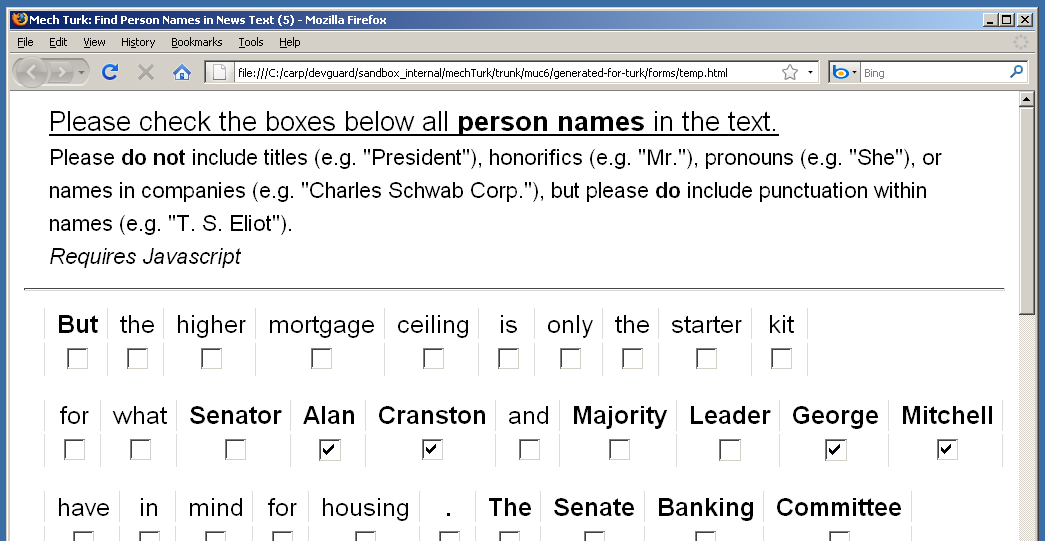
\includegraphics[width=0.95\textwidth]{pngs/big-ne-form.png}


\sld{Named Entities Worked}

\begin{itemize}
\item Conveying the coding standard
\begin{itemize}
\footnotesize
\item official MUC-6 standard dozens of pages
\item examples are key
\end{itemize}

\item Fitts' Law
\begin{itemize}
\footnotesize
\item time to position cursor inversely proportional to target size
\item highlighting text: fine position + drag + position
\item pulldown menus for type: position + pulldown + select
\item checkboxes for entity at a time: fat target click
\end{itemize}
\end{itemize}

\sld{Discussion: Named Entities}

\vspace*{-6pt}
\begin{itemize}
\item 190K tokens, 64K capitalized, 4K person name tokens
\begin{itemize}
\footnotesize
\item 4K / 190K = 2.1\% prevalence of entity tokens
\end{itemize}
\item 10 annotators per token
\item 100+ annotators, varying numbers of annotations
\item Less than a week at 2 cents/400 tokens (US\$95)
\item Aggregated Turkers better than LDC data
\begin{itemize}
\footnotesize
\item Correctly Rejected:
{\tt\footnotesize Webster's, Seagram, Du Pont,
\\
Buick-Cadillac, Moon, erstwhile Phineas Foggs}
\item Incorrectly Accepted: {\tt\footnotesize Tass}
\item Missed Punctuation: {\tt\footnotesize J~E.~``Buster'' Brown}
\end{itemize}

\end{itemize}


\sld{Case 2: Morphological Stemming}

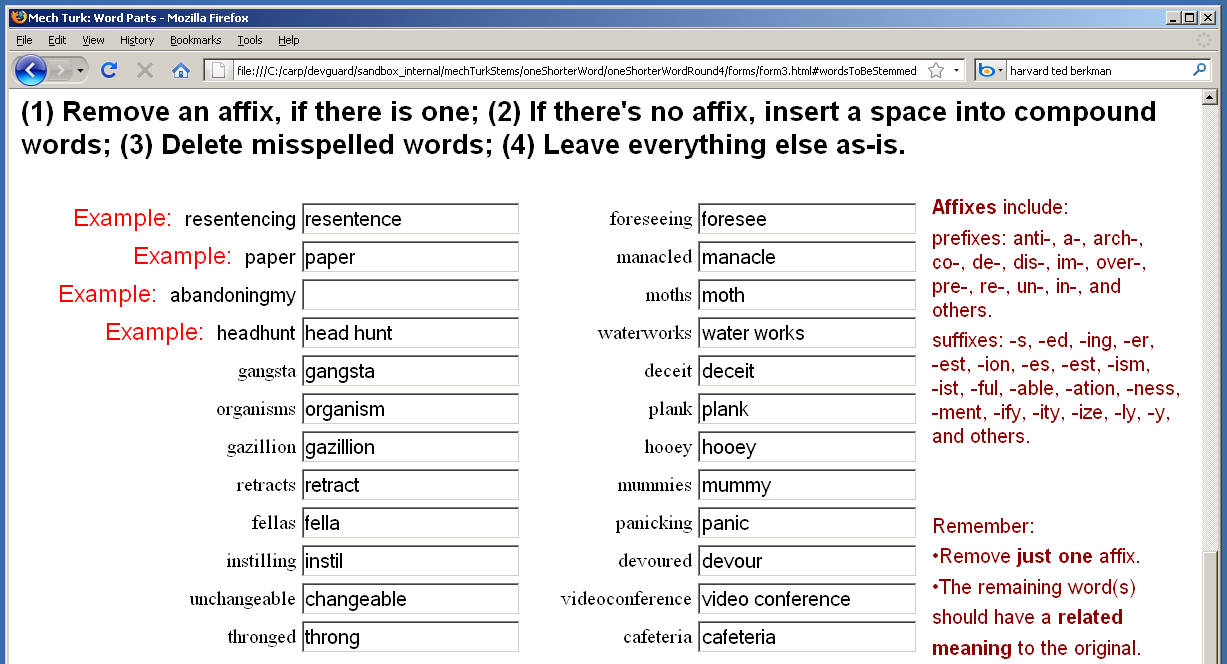
\includegraphics[width=0.95\textwidth]{pngs/stems-v4.png}

\sld{Morphological Stemming Worked}

\begin{itemize}
\vspace*{-8pt}
\item Coded and tested by intern (Emily Jamison of OSU)
\begin{itemize}
\footnotesize
\item Less than one month to code, modify and collect 
\end{itemize}
\item Three iterations of coding standard, Four of instructions
\begin{itemize}
\footnotesize
\item began with full morphological segmentation (too hard)
\item simplified task to one stem with full base (more ``natural'')
\item added previously confusing full examples + affixes
\end{itemize}

\item Added qualifying test

\item 60K (50K frequent Gigaword, 10K random) tokens
\item 5 annotators / token
\end{itemize}




\sld{Case 3: RTE-1}
\begin{itemize}
\item Examples and gold standard by Dagan et al. (2005)
\item 800 Items (400 true, 400 false in gold standard)
\item Used for 1st Recognizing Textual Entailment Bakeoff
\item Examples
\begin{itemize}
\footnotesize
\item
{\it ID:} 56   \ \ \ {\it Gold Label:} TRUE
\\[2pt]
{\it Text:} Euro-Scandinavian media cheer Denmark v Sweden draw.
\\[2pt]
{\it Hypothesis:} Denmark and Sweden tie.
\\
\item
{\it ID:} 77  \ \ \ {\it Gold Label:} FALSE
\\[2pt]
{\it Text:} Clinton's new book is not big seller here.
\\[2pt]
{\it Hypotheis:} Clinton's book is a big seller.
\end{itemize}
\end{itemize}

\sld{Turker Annotations for RTE-1}
\begin{itemize}
\item Collected by Dolores Labs
\item Analyzed by Snow et al. in {\it EMNLP}\ paper
\item They also recreated 4 other NLP datasets:
\begin{itemize} 
\footnotesize 
\item word sense (multinomial)
\item sentiment (multi-faceted scalar 1--100)
\item temporal ordering (binary)
\item word similarity (ordinal 1--10)
\end{itemize}
\item 2 items/task, 10 Turkers per item, 164 Turkers total
\item All five tasks completed in a few days
\item All five tasks cost under US\$100
\end{itemize}

\sld{Turker Instructions for RTE-1}
\begin{itemize}
\item Instructions
\\[6pt]
{\footnotesize Please state whether the
second sentence (the Hypothesis) is implied by the information in
first sentence (the Text), i.e., please state whether the Hypothesis
can be determined to be true given that the Text is true.

Assume that you do not know anything about the situation except what the Text itself says. 

Also, note that every part of the Hypothesis must be implied by the Text in order for it to be true.
}
\item Plus, 2 true and 2 false examples
\end{itemize}

\sld{(Munged) Turker Data for RTE-1}
\begin{verbatim}
           Item   Coder  Label   |     k    i  j  x
  -------------------------------------------------   
     1     i[1]    j[1]   x[1]   |     1    1  1  1   
     2     i[2]    j[2]   x[2]   |     2    1  2  1
     3     i[3]    j[3]   x[3]   |     3    1  3  1
     4     i[4]    j[4]   x[4]   |     4    1  4  0
                                 |
   509   i[509]  j[509]  x[509]  |   509   51  22 0
   510   i[510]  j[510]  x[510]  |   510   51  10 1
   511   i[511]  j[511]  x[511]  |   511   52   4 1
   512   i[512]  j[512]  x[512]  |   512   52   1 1
                                 |
  8000  i[8000] j[8000] x[8000]  |  8000  800 144 1
\end{verbatim}

\sld{Two or More Category Labels}
\begin{itemize}
\item Assume binary categories for simplicity
\begin{itemize}
\footnotesize
\item 0 = ``FALSE'',  1 = ``TRUE'' (arbitrary for task)
\item e.g. Named entities: Token in Name = 1, not in Name = 0
\item e.g. RTE-1: entailment = 1, non-entailment = 0
\item e.g. Information Retrieval: relevant=1, irrelevant=0
\end{itemize}
\item Models generalize to more than two categories
\begin{itemize}
\footnotesize
\item e.g. Named Entities: PERS, LOC, ORG, NOT-IN-NAME
\end{itemize}
\item Models generalize to ordinals or scalars
\begin{itemize}
\footnotesize
\item e.g. Paper Review: 1-5 scale
\item e.g. Sentiment: 1-100 scale of positivity
\end{itemize}
\end{itemize}

\sld{Prevalence}
\begin{itemize}
\item Assumes binary categories (0 = ''FALSE'', 1 = ''TRUE'')
\item Prevalence = \% of 1 labels
\begin{itemize}
\footnotesize
\item e.g. RTE-1 400/800 = 50\%  \ [artificially ``balanced'']
\item e.g. Bridging anaphors (among all anaphors): 6\%
\item e.g. Person named entity tokens 4K / 190K = 2.1\%
\item e.g. Zero (tennis) sense of ``love'' in newswire: 1\% 
\item e.g. Relevant docs for web query [Malta LREC]: \\
\hspace*{36pt}500K/1T = 0.00005\%
\end{itemize}
\end{itemize}

\sld{Sensitivity and Specificity}
\begin{itemize}
\item Assume binary categories (0=''false'', 1=''true'')
\item Reference is gold standard, Response from coder
\item 
\begin{tabular}{|r|l|l|}
\hline
      & Resp=1 & Resp=0 \\ 
\hline
Ref=1 & TP     & FN  \\ 
\hline
Ref=0 & FP     & TN \\ 
\hline
\end{tabular}
\item Sensitivity = TP/(TP+FN) \ \ {\footnotesize = Recall}
\begin{itemize}
\footnotesize
\item Accuracy on 1 (true) items
\end{itemize}
\item Specificity = TN/(TN+FP) \ \ {\footnotesize $\neq$ Precision = TP/(TP+FP)}
\begin{itemize}
\footnotesize
\item Accuracy on 0 (false) items
\end{itemize}
\end{itemize}

\sld{Generative Labeling Model}
\vspace*{-8pt}
\begin{itemize}
\item Item $i$'s category $c_i \in \{ 0, 1 \}$
\item Coder $j$'s specificity $\theta_{0,j} \in [0,1]$; \ sensitivity $\theta_{1,j} \in [0,1]$
\item Coder $j$'s label for item $i$: $x_{i,j} \in \{ 0, 1 \}$
\item If category $c_i=1$,
\begin{itemize}
\footnotesize
\item $\mbox{\rm Pr}(x_{i,j}=1) = \theta_{1,j}$ \ \ [correctly labeled]
\item $\mbox{\rm Pr}(x_{i,j}=0) = 1 - \theta_{1,j}$
\end{itemize}
\item If category $c_i=0$, 
\begin{itemize}
\footnotesize
\item $\mbox{\rm Pr}(x_{i,j}=1) = 1 - \theta_{0,j}$ 
\item $\mbox{\rm Pr}(x_{i,j}=0) = \theta_{0,j}$ \ \ [correctly labeled]
\end{itemize}
\item $\mbox{\rm Pr}(x_{i,j}=1|c,\theta) = c_i \theta_{1,j} + (1 - c_i) (1 - \theta_{0,j})$
\end{itemize}

\sld{Calculating Category Probabilities}
\begin{itemize}
\item Bayes's Rule 
\\[4pt]
$\begin{array}{rcl}
p(a|b) 
& =       & p(b|a) \ p(a) / p(b) 
\\[4pt]
& \propto & p(b|a) \ p(a)
\end{array}$
\item Applied to Category Probabilities
\\[4pt]
$\begin{array}{rcl}
p(c_i|x_i,\theta,\pi) 
& \propto & p(x_i|c_i,\theta,\pi) \ p(c_i|\theta,\pi) 
\\[4pt]
& = & p(x_i|c_i,\theta) \ p(c_i|\pi)
\\[4pt]
& = & p(c_i|\pi) \ \prod_{j=1}^J p(x_{i,j}|c_i,\theta)
\end{array}$
\end{itemize}

\sld{Calculating Cat Probabilities: Example}

\begin{itemize}
\footnotesize
\item Prevalence: \ $\pi = 0.2$
\item Specificities: \  $\theta_{0,1} = 0.60$; \ \ $\theta_{0,2} = 0.70$; \ \ $\theta_{0,3} = 0.80$
\item Sensitivities: \ $\theta_{1,1} = 0.75$; \ \ $\theta_{1,2} = 0.65$; \ \ $\theta_{1,3} = 0.95$
\item Annotations for item $i$: \ $x_{i,1} = 1$, \ $x_{i,2} = 1$, \ $x_{i,3} = 0$
\\[8pt]
\hspace*{-12pt}$\begin{array}{rcl}
\footnotesize
\mbox{\rm Pr}(c_i=1|\theta,x) 
& \propto & \pi \ \mbox{\rm Pr}(x_i=\langle 1,1,0 \rangle | \theta,c_i=1)
\\[4pt]
& = & 0.2 \cdot 0.75 \cdot 0.65 \cdot (1 - 0.95) = 0.004875
\end{array}$
\\[8pt]
\hspace*{-12pt}
$\begin{array}{rcl}
\footnotesize
\mbox{\rm Pr}(c_i=0|\theta,x) 
& \propto & (1 - \pi) \ \mbox{\rm Pr}(x_i=\langle 1,1,0 \rangle | \theta,c_i=0)
\\[4pt]
& = & (1 - 0.2) \cdot (1 - 0.6) \cdot (1 - 0.7) \cdot (1 - 0.8) = 0.0192
\end{array}$
\\[8pt]
\hspace*{-8pt}$\mbox{\rm Pr}(c_i=1|\theta,x) = 0.004875 / (0.004875 + 0.0192) = 0.2024922$
\end{itemize}

\sld{Bayesian Models}
\begin{itemize}
\footnotesize
\item Observed data: \ $y$; \ \ \ Model parameter(s): \ $\phi$
\item Likelihood function (or sampling distribution): \ $p(y|\phi)$
\item Prior: \ $p(\phi)$
\item Chain rule: \ $p(y,\phi) = p(y|\phi) \ p(\phi)$
\item Marginal (prior predictive distribution): \ $p(y) = \int p(y|\phi) \ p(\phi) \ d\phi$
\item Posterior: $p(\phi|y)$ calculated via Bayes's rule
\\[4pt]
$\begin{array}{rcl}
p(\phi|y) & = & p(y,\phi) / p(y)
\\[4pt]
& = & p(y|\phi) \ p(\phi) / p(y)  
\\[4pt]
& = & p(y|\phi) \ p(\phi) / \int p(y | \phi') p(\phi') d\phi'
\\[4pt]
& \propto & p(y|\phi) \ p(\phi)
\end{array}
$
\end{itemize}

\sld{Point Estimators are ``Best'' Guesses}
\footnotesize
\begin{itemize}
\item Estimate parameters $\phi$ given observed data $y$
\item Maximum Likelihood Estimator (ML) 
\\[4pt]
$\phi^{*}(y) = \arg\max_\phi p(y|\phi)$
\\[4pt]
maximizes probability of observed data given parameters
\item Maximum a Posteriori (MAP) Estimate 
\\[4pt] 
$\hat{\phi}(y) = \arg\max_\phi p(\phi|y) = \arg\max_\phi p(y|\phi) \ p(\phi)$
\\[4pt]
maximizes probability of parameters given observed data
\item If prior is constant, [i.e. $p(\phi) = c$], then $\hat{\phi}(y) = \phi^{*}(y)$
\item Bayesian estimator is expected parameter values given observed data
\\[4pt]
$\bar{\phi}(y) = \mathbb{E}[\phi] = \int \phi \ p(\phi|y) \ d\phi$
\item Bayesian estimates are unbiased [i.e. estimate equals expection] by definition
\end{itemize}

\sld{Inference}
\footnotesize
\begin{itemize}
\item Observed data $y$; \ \ New data $\tilde{y}$
\item Posterior predictive distribution: \ $p(\tilde{y}|y)$
\item Maximum likelihood approximation: \ $p(\tilde{y}|y) \approx p(\tilde{y}|\phi^*(y))$
\item MAP approximation: \ $p(\tilde{y}|y) \approx p(\tilde{y}|\hat{\phi}(y))$
\item Bayesian point approximation: \ $p(\tilde{y}|y) \approx p(\tilde{y} | \bar{\phi}(y))$
\item Bayesian posterior predictive distribution
\\[4pt]
$p(\tilde{y}|y) = \int p(\tilde{y}|\phi) \ p(\phi|y) \ d\phi$
\\[4pt]
averages over uncertainty in estimate of $\phi$ [i.e. $p(\phi|y)$]
\end{itemize}

\sld{Bernoulli Distribution (Single Binary Trial)}
\begin{itemize}
\item Outcome $y \in \{ 0, 1 \}$ \ \ [success=1, failure=0]
\item Parameter $\theta \in [0,1]$ is chance of success 
\item 
$p(y|\theta)
= \mbox{\sf Bernoulli}(y|\theta) 
= \theta^y \ (1 - \theta)^{1-y}
=
\begin{cases}
\theta & \mbox{if } $y = 1$
\\
1 - \theta & \mbox{if } $y = 0$
\end{cases}$
\vspace*{6pt}
\item
For $N$ independent trials $y = y_1,\ldots,y_N$, \ where $y_n \in \{ 0, 1 \}$,
\\[4pt]
$\begin{array}{rcl}
p(y|\theta) & = & \prod_{n = 1}^N p(y_n|\theta)
\\[4pt]
& = & \prod_{n=1}^N \theta^{y_n} \ (1-\theta)^{1-y_n}
\\[4pt]
& = & \theta^A (1-\theta)^B
\end{array}$
\\[4pt]
where $A = \sum_{n=1}^N y_n$ and $B = \sum_{n=1}^N (1 - y_n) = N - A$
\\[4pt]
\vfill
\item
{\scriptsize $x^0 = 1$ \ \ and \ \ $x^a x^b = x^{a+b}$}
\end{itemize}

\sld{Conjugate Priors}
\begin{itemize}
\item Given a sampling distribution $p(y|\phi)$
\item Given a family of distributions $\mathcal{F}$
\item The family $\mathcal{F}$ is conjugate for $p(y|\phi)$ if
\\[4pt]
prior $p(\phi) \in \mathcal{F}$ implies posterior $p(\phi|y) \in \mathcal{F}$
\item Provides analytic form of posterior (vs.\ numerical approximation)
\item Supports incremental updates
\begin{itemize}
\item Start with prior $p(\phi) \in \mathcal{F}$
\item After data $y$, have posterior $p(\phi|y) \in \mathcal{F}$
\item Use $p(\phi|y)$ as prior for new data $y'$
\item New posterior is $p(\phi|y,y') \in \mathcal{F}$
\item i.e.\ updating with $y$ then $y'$ same as upating for $y,y'$ together
\end{itemize}
\item Not necessary for Bayesian inference
\end{itemize}

\sld{Mean, Mode and Variance for Bernoulli}

\begin{itemize}
\item Mean and Mode: \ $\mathbb{E}[\mbox{\sf Bern}(\theta)] = \mbox{\rm mode}[\mbox{\sf Bern}(\theta)] = \theta$
\item Variance: \ $\mbox{\rm var}[\mbox{\sf Bern}(\theta)] = \theta \ (1-\theta)$
\item Standard Deviation: \ $\mbox{\rm sd}[\mbox{\sf Bern}(\theta)] = \sqrt{\theta \ (1-\theta)}$
\vfill
\item {\scriptsize For discrete $X$ with $N$ outcomes $x_1,\ldots,x_N$ distributed $p_X(x)$}
\begin{itemize}
\scriptsize
\item Mode (Max Value): \ $\mbox{\rm mode}[X] = \arg\max_{n=1}^N p(x_n)$
\item Mean (Average Value): \ $\mathbb{E}[X] = \sum_{n=1}^N p(x_n) \ x_n $
\item Variance: \ $\mbox{\rm var}[X] = \mathbb{E}[X-\mathbb{E}[X]] = \sum_{n=1}^N p(x_n) \ (x_n - \mathbb{E}[X])^2$
\item Standard Deviation: \ $\mbox{\rm sd}[X] = \sqrt{\mbox{\rm var}[X]}$
\end{itemize}
\end{itemize}

\sld{Beta Distribution}
\begin{itemize}
\item Outcome $\theta \in [0,1]$
\item Parameters $\alpha,\beta > 0$
\ \ \ [$\alpha-1$ prior successes; $\beta-1$ failures]
\item 
Continuous Density Function
\\[4pt]
$\begin{array}{rcl}
p(\theta|\alpha,\beta) 
& = & \mbox{\sf Beta}(\theta|\alpha,\beta)
\\[8pt]
& = & \frac{1}{\displaystyle \mbox{\rm B}(\alpha,\beta)} \ \ \theta^{\alpha-1} \ (1-\theta)^{\beta-1}
\\[8pt]
& \propto & \theta^{\alpha-1} \ (1-\theta)^{\beta-1}
\end{array}$
\vfill
\item {\scriptsize
Continuous densities $p(\theta)$ have $p(\theta) \geq 0$ and $\int p(\theta) d\theta = 1$
}
\item {\scriptsize
Beta function $\mbox{\rm B}(\alpha,\beta) = \int_0^1 \theta^{\alpha-1} \ (1-\theta)^{\beta-1} \ d\theta 
=  \frac{\Gamma(\alpha+\beta)}{\Gamma(\alpha)\Gamma(\beta)}$}
\item {\scriptsize
$\Gamma(x) = \int_0^{\infty} y^{x-1} \ \exp(-y) dy$ \ \ is continuous generalization of factorial
\\[4pt]
i.e. $\Gamma(n+1) = n! = n \times (n-1) \times \cdots\times 2 \times 1$ \ for integer $n \geq 0$}
\end{itemize}

\sld{\normalsize Beta Examples}

\vspace*{-8pt}
% 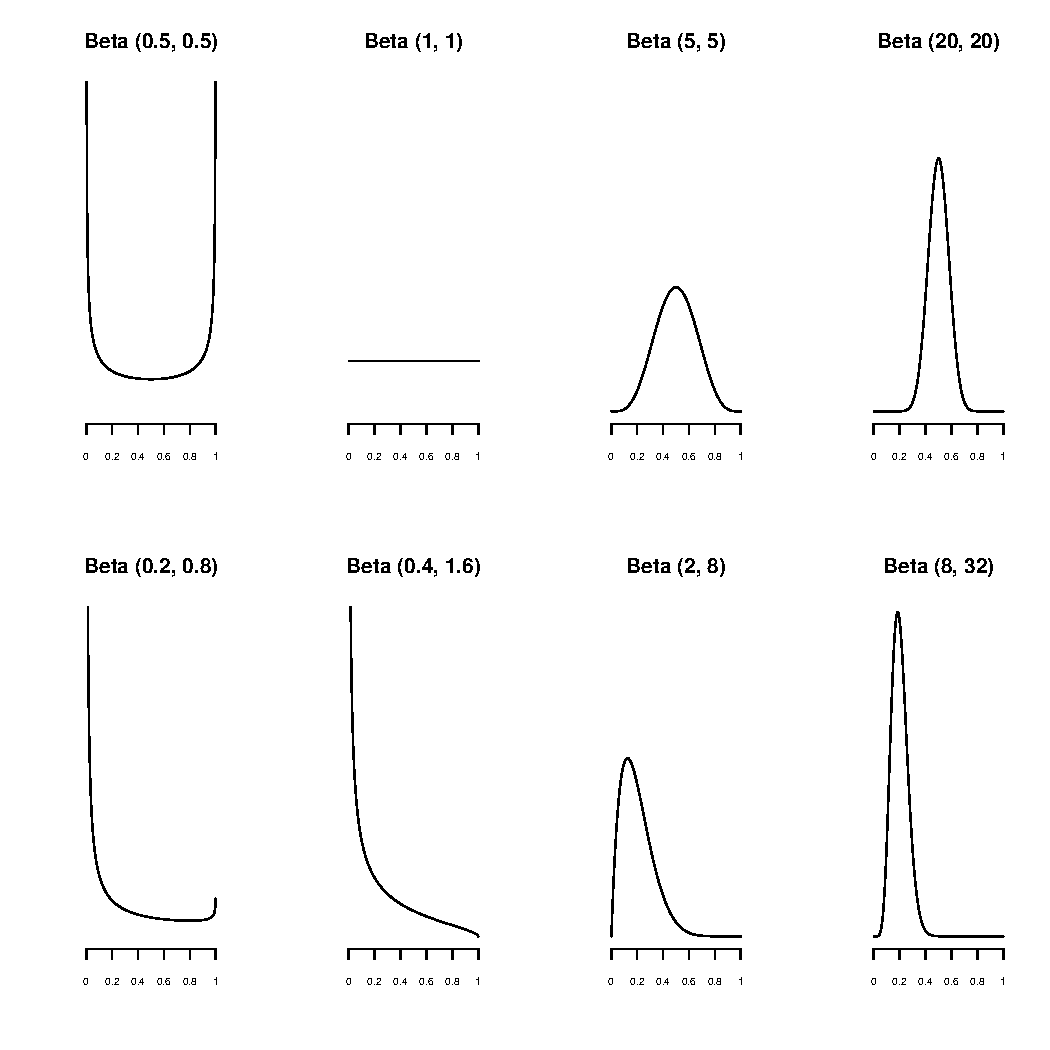
\includegraphics[width=0.65\textwidth]{pdf/beta-examples.pdf}
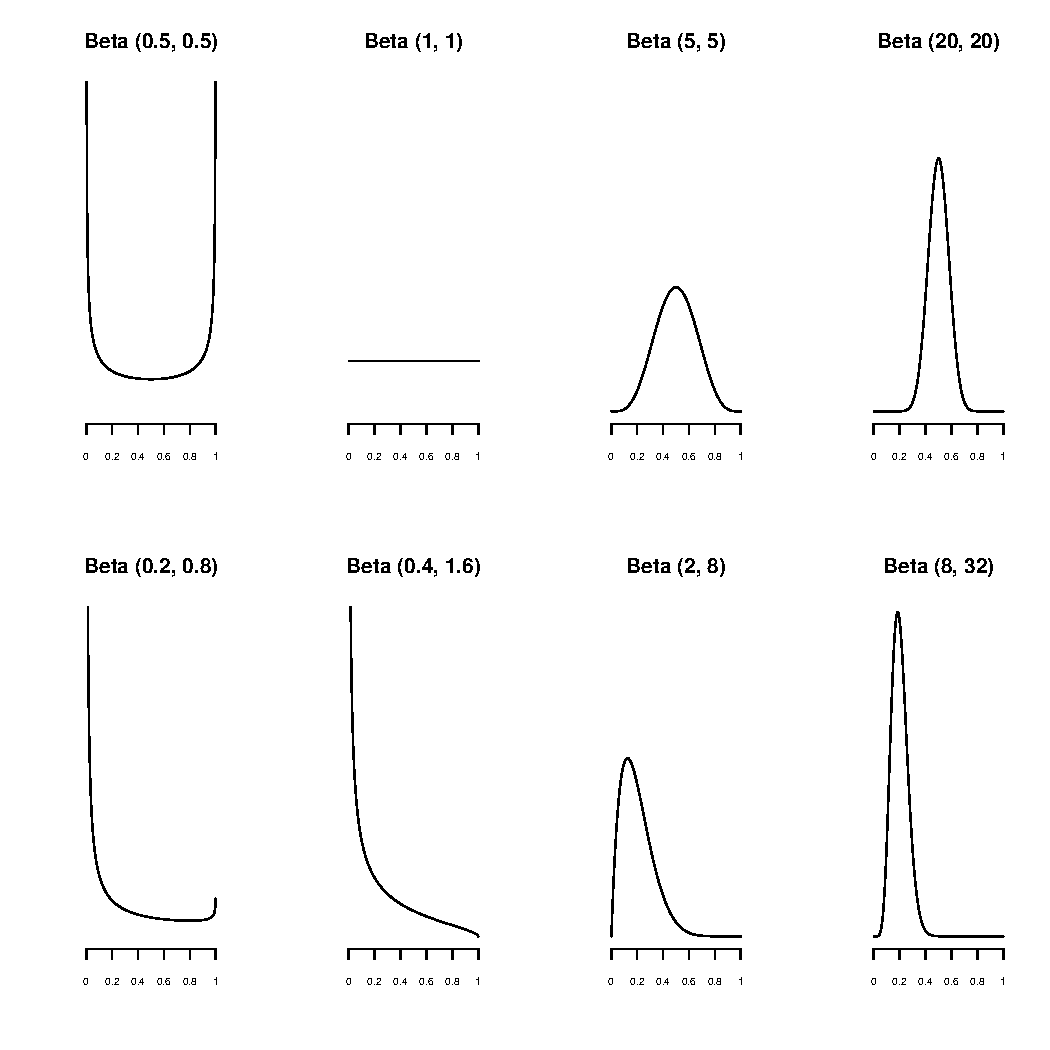
\includegraphics[height=1.0\textheight,width=0.85\textwidth]{pdf/beta-examples.pdf}


\sld{Mean, Mode and Variance for Beta}
\begin{itemize}
\item Mean: \ 
$\mathbb{E}[\mbox{\sf Beta}(\alpha,\beta)] = \frac{\displaystyle \alpha}{\displaystyle \alpha+\beta}$
\item Variance: \ 
$\mbox{\rm var}[\mbox{\sf Beta}(\alpha,\beta)] = \frac{\displaystyle \alpha\beta}{\displaystyle (\alpha+\beta)^2 \ (\alpha + \beta + 1)}$
\item Mode: \ 
$\mbox{\rm mode}[\mbox{\sf Beta}(\alpha,\beta)] 
= 
\begin{cases} 
\frac{\displaystyle \alpha-1}{\displaystyle \alpha+\beta-2} & \mbox{if } \alpha > 1 \mbox{ and } \beta > 1
\\[4pt]
\mbox{undefined} & \mbox{otherwise}
\end{cases}$
\end{itemize}


\sld{Beta is Conjugate Prior for Bernoulli}
\begin{itemize}
\item Data $y = y_1,\ldots,y_N$ for $y_n \in \{ 0, 1 \}$
\item Prior $p(\theta) = \mbox{\sf Beta}(\theta|\alpha,\beta)$
\item Likelihood $p(y|\theta) = \prod_{n=1}^N \mbox{\sf Bern}(y_n|\theta) = \theta^A (1-\theta)^B$
\\[4pt] {\scriptsize where $A$ is number of successes, $B$ number of failures in $y$}
\item Posterior 
$\begin{array}{rcl}
p(\theta|y) & \propto & p(y|\theta) \ p(\theta)
\\[4pt]
& = & \prod_{n=1}^N \mbox{\sf Bern}(y_n|\theta) 
\end{array}$
\end{itemize}

\end{document}
